\documentclass[a4paper,10pt]{article}
% Intento aprovechar un poco mas toda la hoja.
\usepackage[cm]{fullpage}
%%%%%%%%%%%%%%%%%%%%%%%%%%%%%%%%%%%%%%%%%%%%%%%%%%%%%%%%%%%%%%%%%
% Paquetes de fuentes:
% Input encoding.
\usepackage[utf8]{inputenc}
% Ver pagina 92 de "The not so short introduction to Latex" por Tobias Oetiker
% para entender que hacen estos paquetes.
\usepackage{lmodern}
\usepackage[T1]{fontenc}
\usepackage{textcomp}
\usepackage{listings}



\usepackage{vmargin}
\setpapersize{A4}
\setmargins{4.5cm}       % margen izquierdo
{1.5cm}                        % margen superior
{13.5cm}                      % anchura del texto
{23.42cm}                    % altura del texto
{10pt}                           % altura de los encabezados
{1cm}                           % espacio entre el texto y los encabezados
{0pt}                             % altura del pie de página
{2cm}                           % espacio entre el texto y el pie de página

% Paquetes para matematica:
\usepackage{amsmath}
	% Formato de numeracion de ecuaciones por seccion. Ej. seccion x, ecuacion y: (x.y)
	\numberwithin{equation}{section}
	\numberwithin{figure}{section}
	% Simbolos matematicos. Por ej. la 'R' de reales, etc...
	\usepackage{amssymb}

% Paquete para graficos:
\usepackage{graphicx}

% Paquete que deja sangria luego de comenzada una seccion nueva.
\usepackage{indentfirst}

\usepackage{color}
\usepackage{fancyvrb}
\usepackage{float}
% Paquete para hacer subrayados, poner textos en color y resaltar texto en color.
% Lo bueno de este paquete es que no tira errores de fullbox como cuando se usa \colorbox{declared-color}{text}.
% El unico problema es que no soporta acentos desde el teclado (tira un error de UTF8). Hay que incluirlos usando \'.
\usepackage{soul}

% Paquete para incluir codigo fuente de MatLab cuando sea necesario.
%\usepackage[numbered,autolinebreaks]{mcode}

% Incluir la bibliografia en la tabla de contenidos.
\usepackage[nottoc,numbib]{tocbibind}

%\usepackage{mcode}
\usepackage{booktabs}
\usepackage{multirow}
% Paquete para utilizar hipertexto (tiene que ser siempre el ultimo paquete que se carga).
% Todos los links, referencias, etc...pasan a ser hipertextos.
\usepackage[pdftex]{hyperref}
% Setup del paquete de hipertexto.
\hypersetup{pdftitle = {75.12 TP2} }
\hypersetup{colorlinks = false}
\hypersetup{%
    pdfborder = {0 0 0}
}
\usepackage{booktabs}		%Permiten manejar mejor el tamaño de las tablas
\usepackage{tabulary}		%Permiten manejar mejor el tamaño de las tablas
\begin{document}

% Carátula:
\begin{titlepage}

\thispagestyle{empty}

\begin{center}

\large{\textsc{Universidad de Buenos Aires}}\\
\large{\textsc{Facultad de Ingeniería}}\\
\small{Año 2018 - 2\textsuperscript{do} Cuatrimestre}
\end{center}

\vfill

\begin{center}
\Large{\underline{\textsc{66.20 Organización de Computadoras - Práctica Jueves}}}
\end{center}

\vfill

\begin{tabbing}
\hspace{2cm}\=\+TRABAJO PRÁCTICO 1: conjunto de instrucciones MIPS\\
	FECHA DE ENTREGA: 11 de Octubre de 2018\\
\\
	INTEGRANTES:\hspace{-1cm}\=\+\hspace{1cm}\=\hspace{6cm}\=\\
		BURASTERO, Maximiliano	\>\>- \ 94508\\
			\>\footnotesize{$<$maxicc4@gmail.com$>$}\\
		PEREZ ONDARTS, Flavio	\>\>- \ 96786\\
			\>\footnotesize{$<$perezflavio94@gmail.com$>$}\\
		YACOBUCCI, Maximiliano	\>\>- \ 93321\\
			\>\footnotesize{$<$maxyacobucci@gmail.com$>$}\\
\end{tabbing}

\vfill

\hrule
\vspace{0.2cm}

\noindent\small{66.20 - Organización de Computadoras - Práctica Jueves}

\end{titlepage}

\newpage





\section{Introducción}

En este trabajo práctico se busca aprender, practicar y perfeccionar los conocimientos relacionados al conjunto de instrucciones MIPS y el concepto de ABI.

El programa será realizado en lenguaje C a excepción de una función (quicksort) que tendrá dos versiones: una MIPS32 y una en C. El mismo se ejecutará teniendo en cuenta los parámetros que se se especifiquen por consola.



\section{Diseño e Implementación}

\subsection{Diseño}

El programa consiste en una implementación del algoritmo Quicksort, recibiendo como argumento el archivo que contiene datos que se desean ordenar (se asume que cada cadena de caracteres a ordenar aparece de a una por línea), y devolviendo por stdout los valores ordenados. En caso de errores, se devuelven por stderr. 

Asimismo, el programa contará con una sección de ayuda que mostrará las opciones disponibles. El usuario que lo utilice deberá ingresar por línea de comando una serie de parámetros describiendo el archivo que contiene los datos y el archivo de salida, pudiendo indicar si se quiere ordenar números.

Es importante destacar que el programa será portable, teniendo una versión del algoritmo quicksort en C y otra en MIPS32 para dar soporte geńerico a aquellos entornos que carezcan de una versión
más espećıfica .El programa será compilado y posteriormente enlazado usando herramientas de GNU disponibles en el sistema NetBSD, generando una aplicación ejecutable.


\subsection{Implementación}

Inicialmente el programa revisa los parámetros indicados por línea de consola. En caso de no haber errores en ellos se procede a correr el algoritmo correspondiente. Si se solicita ayuda se mostrará el cartel con los comandos disponibles. Si se quiere averiguar la versión del programa, el mismo cuenta con una opción para indicarla. Si en cambio se indicó un archivo para ser ordenado, procederá a leerlo. Si no se indica un archivo de salida, se usará la salida estándar (stdout).

Luego de leer el archivo se procede a llamar al algoritmo de quicksort. Como se comentó anteriormente, existen 2 versiones del mismo, una en lenguaje C y otra en MIPS32. Ambos contienen su propia función atoi. En el algoritmo se usan punteros a char siendo identificado el primero como izq y el último como der. En el caso del algoritmo en lenguaje Assembler se hizo uso de la ABI, almacenando por el callee a los argumentos correspondientes a los registros a0-a3.

Por último, se libera la memoria utilizada y se imprimen en pantalla por stdout los datos ordenados.


A continuación se adjuntan porciones del código assembly, junto con un diagrama de su stack.


\subsubsection{Código Assembly Quicksort}
\setmargins{2cm}{1.5cm}{13.5cm}{23.42cm}{10pt}{1cm}{0pt}
{2cm}
\begin{lstlisting}[language=c, numbers=none]
## void quicksort(char** a, char** b, int mum);
quicksort:
    ## if (a>b) return;
    bgt		a0, a1, fin_quicksort	# if a0 > a1 then fin_quicksort  
##Prologo
    addiu   sp,sp,-32     #stack frame de 8 palabras
    sw      fp,24(sp)
    move    fp,sp
    sw      s0,16(fp)     #en s0 guardaremos el resultado de partition
    sw      gp,20(fp)     
    sw      ra,28(fp)     #Guardamos la direccion de retorno
    ##Guardamos los argumentos en el stackframe del caller
    sw      a0,32(fp)
    sw      a1,36(fp)
    sw      a2,40(fp)
    jal     partition
    move    s0,v0         #s0 = char** x = partition(a,b,num)
    lw      a0,32(fp)     
    addi    a1,v0,-4
    lw      a2,40(fp)
    jal     quicksort       #quicksort(a,x-1,num) (x = v0)
    addi    a0,s0,4
    lw      a1,36(fp)
    lw      a2,40(fp)
    jal     quicksort       #quicksort(x+1,b,num)
##Epílogo
    lw      s0,16(fp)
    lw      gp,20(fp)
    lw      ra,28(fp)
    move    sp,fp
    lw      fp,24(sp)
    addiu   sp,sp,32
fin_quicksort:
    jr		ra					# jump to ra

\end{lstlisting}

\begin{figure}[h]
  \centering
    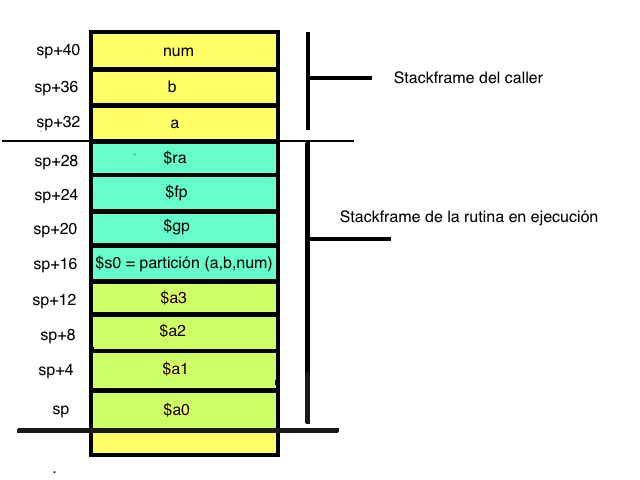
\includegraphics[width=1\textwidth]{quicksort_stack.png}
  \caption{Stack frame utilizado en quicksort}
  \label{fig:stack}
\end{figure}



\subsubsection{Código Assembly Partition}
\begin{lstlisting}[language=c, numbers=none]
## char** partition(char** a, char** b, int num)
partition:
##Prólogo
    addiu   sp,sp,-40    #stack frame de 10 palabras
    
    sw      fp, 32(sp)   
    move    fp, sp
    sw		s0, 16(fp)	  # en s0 guardaremos el pivot	
    sw      s1, 20(fp)    # en s1 guardaremos un contador i
    sw      s2, 24(fp)    # en s2 guardaremos un contador j
    sw      gp, 28(fp)
    sw      ra, 36(fp)    # guardamos la direccion de retorno
    
    ##guardamos los argumentos en el stackframe del caller
    sw      a0, 40(fp)    
    sw      a1, 44(fp)
    sw      a2, 48(fp)

    lw      s0, 0(a1)     # s0 = pivot (char*)
    li		s1, -4		    # s4 = i = -1 
    li		s2, 0		    # s5 = j = 0
    beq     a2, 0, loop   # si num==0 vamos al loop sin atoi al pivot
pivot_entero:
    move    a0,s0
    jal     mi_atoi
    move    s0,v0
loop:
    ##cargamos los argumentos desde el stackframe del caller
    lw      a0, 40(fp)        
    lw      a1, 44(fp)
    lw      a2, 48(fp)
    
    add		t0, s2, a0		# t0 = (char**) &a[j]
    beq     t0, a1, fin       # si &a[j] == b then fin
    lw      a1, 0(t0)         # a1 = (char*) a[j]
    move    a0, s0            # a0 = pivot
    beq     a2, 0, alfa       # si num == 0 comparar alfabeticamente
    move    a0, a1            # convertir a[j] en int
    jal     mi_atoi
    move 	a1,v0		        # a1 = v0 = atoi(a[j])
    move    a0,s0             # a0 = pivot (otra vez)
    jal		cmp_int             # cmp_int(int pivot,int a[j]);
    nop
    b		swap_decision			# branch to swap_decision
alfa:
    jal     cmp_alfa            #cmp_alfa(char*pivot,char*a[j]);

                                #cmp(pivot,a[j]): = 0 si pivot>=a[j]|| 1 si a[j]>pivot
swap_decision:
    bgt		v0,0, next	# si pivot >= a[j] hay swap, si no, next
    lw      a0, 40(fp)    # a0 = a
    addi    s1,s1,4   # i+=1
    add     a1,a0,s1 # a1 = &a[i]
    add     a0,a0,s2 # a0 = &a[j]
    jal     swap        # swap(char**&a[j],char**&a[i]);
    nop
next:
    addi    s2,s2,4   # j+=1
    b		loop		# branch to loop
fin:
    addi    s1,s1,4       # i+=1
    add     a0,a0,s1     # a0 = &a[i]
    jal     swap            # swap(char** a[i], char** &pivot);
    nop
    lw      a0, 40(fp)
    add     v0, a0, s1    #return &a[i] = a + i
##Epílogo
    lw		s0, 16(fp)	#reponemos el stack 
    lw      s1, 20(fp)
    lw      s2, 24(fp)
    lw      gp, 28(fp)
    lw      ra, 36(fp)
    move    sp,fp
    lw      fp,32(sp)
    addiu   sp,sp,40
    jr		ra				# jump to ra
    
\end{lstlisting}

\begin{figure}[h]
  \centering
    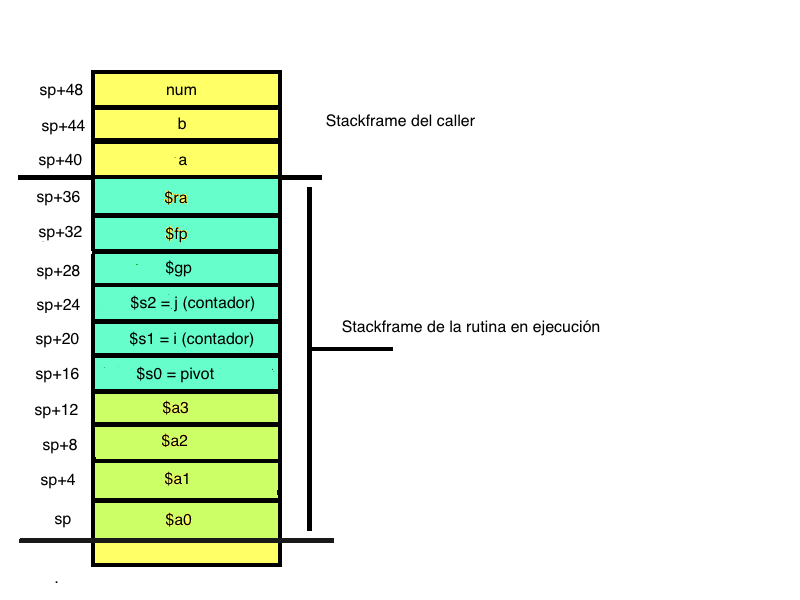
\includegraphics[width=1\textwidth]{partition_stack.png}
  \caption{Stack frame utilizado en partition}
  \label{fig:stack}
\end{figure}

\setmargins{4.5cm}{1.5cm}{13.5cm}{23.42cm} {10pt}{1cm}{2cm}    

\section{Comando para compilar el programa} 

En primer lugar para compilar el programa se debe abrir una consola, pararse en la carpeta correspondiente al programa y ejecutar la siguiente sentencia para compilarlo:

\begin{center}
gcc -std=c99 -o qsort main.c quicksort.S
\end{center}

En caso que se quiera utilizar la versión del algoritmo de quicksort en C:

\begin{center}
gcc -std=c99 -o qsort main.c quicksort.c
\end{center}


Luego se lo puede ejecutar en cualquiera de sus 3 usos:

\begin{enumerate}
	\item "./qsort -h": muestra la ayuda que indica las diferentes formas de ejecutar el programa 
	\item "./qsort -V": muestra la versión del programa
	\item "./qsort [options] archivo"; ejercuta el programa teniendo como entrada el archivo indicado
\end{enumerate}


En este último caso de uso se pueden indicar las siguiente opciones:

\begin{enumerate}
	\item -o, --output: Archivo de salida
	\item -n, --numeric: Para ordenar los datos numéricamente en vez de alfabéticamente
\end{enumerate}


\section{Resultados obtenidos}


A continuación se mencionarán algunas pruebas realizadas con sus correspondientes resultados. Recordar previamente compilar el programa tal como se explicó en la sección anterior.

\begin{itemize}
\item  ./qsort -h
\end{itemize}
\noindent\fbox{%
    \parbox{\textwidth}{%
        Usage:
        
            ./qsort -h
            
            ./qsort -V
            
            ./qsort [options] archivo
            
        Options:
            
            -h, --help  Imprime ayuda.
            
            -V, --version  Version del programa.
            
            -o, --output  Archivo de salida.
            
            -n, --numeric  Ordenar los datos numericamente en vez de alfabeticamente.
        
        Examples:
            
            ./qsort -n numeros.txt
    }%
}
	

\begin{itemize}
\item  ./qsort -V
\end{itemize}
\noindent\fbox{%
    \parbox{\textwidth}{%
        1.0
    }%
}

\begin{itemize}
\item  ./qsort numeros.txt (conteniendo este archivo 10 numeros del 1 al 10 desordenados)
\end{itemize}
\noindent\fbox{%
    \parbox{\textwidth}{%
        1
        
        10
        
        2
        
        3
        
        4
        
        5
        
        6
        
        7
    
        8
        
        9
    }%
}

Como se puede observar, los números salieron ordenados alfabeticamente, estando el 10 luego del 1.

\begin{itemize}
\item  ./qsort -n numeros.txt 
\end{itemize}
\noindent\fbox{%
    \parbox{\textwidth}{%
        1
        
        2
        
        3
        
        4
        
        5
        
        6
        
        7
    
        8
        
        9
        
        10
    }%
}

En este caso los números se ordenaron numéricamente, estando el 10 luego del 9.

\begin{itemize}
\item  ./qsort text1.txt 
\end{itemize}
\noindent\fbox{%
    \parbox{\textwidth}{%
        aaaaaaa
        
        aaaaaaa
        
        aaaaaaa a
        
        aaaaaaa b
        
        aaaaaaaaaaaaaaaaaaaaaaaaaaaaaaaaaa
        
        hola 
        
        que 
        
        tal 
    }%
}

Aquí se observa que el programa ordenó el archivo alfabéticamente, teniendo en cuenta también el texto siguiente al espacio en una línea. Lo mismo sucederá en el siguiente ejemplo.

\begin{itemize}
\item  ./qsort zeta.txt 
\end{itemize}
\noindent\fbox{%
    \parbox{\textwidth}{%
        zzzzzzzzzzzz a
        
        zzzzzzzzzzzz b
        
        zzzzzzzzzzzz sabia que Asuntos Internos le tendia una trampa
    }%
}


\begin{itemize}
\item  ./qsort archivoInexistente.txt 
\end{itemize}
\noindent\fbox{%
    \parbox{\textwidth}{%
cannot open input file.
    }%
}

Al no existir el archivo indicado en la instrucción, el programa tira un error descripivo.

\begin{itemize}
\item  ./qsort vacio.txt 
\end{itemize}
\noindent\fbox{%
    \parbox{\textwidth}{%
Error. Empty file.
    }%
}


\section{Conclusiones}

En este trabajo práctico hemos aprendido a combinar programación en C con MIPS32 logrando una portabilidad que puede ser importante en caso de ser necesario. Asimismo, pudimos observar cómo un algoritmo realizado en C, puede traducirse en Assembler, viendo detalladamente como surgen las distintas instrucciones. Relacionado a esto último, se hizo uso de la ABI, almacenando por el callee a los argumentos correspondientes a los registros a0-a3, comprendiendo la importancia de su uso.
Otra conclusión que pudimos obtener del trabajo práctico es que el uso de la programación en assembler, por lo menos en el alcance de este trabajo práctico presenta muchas desventajas en relación con el lenguaje C, sobre todo lo que respecta al mantenimiento del código. Una modificación
al codigo fuente que en lenguaje C podía llevarnos un esfuerzo insignificante, en assembler se vuelve más complicada debido principalmente a la dificil legibilidad del código.



\section{Apéndice}
\subsection{Codigo fuente\footnote{Se encuentra el formato digitalizado en: https://github.com/maxicc4/quicksort}}
\setmargins{2cm}{1.5cm}{13.5cm}{23.42cm}{10pt}{1cm}{0pt}
{2cm}
\subsubsection{main.c}
\begin{lstlisting}[language=c, numbers=none]
#include <math.h>
#include <stdlib.h>
#include <string.h>
#include <stdio.h>
#include <getopt.h>
#include <sys/stat.h>
#include <errno.h>

#ifndef VERSION
#define VERSION "1.0"
#endif

#ifndef no_argument
#define no_argument 0
#endif

#ifndef required_argument
#define required_argument 1
#endif

#ifndef optional_argument
#define optional_argument 2
#endif

extern void quicksort(char** izq, char** der, int num);

/*
 * Parametros globales.
 */

FILE *output = NULL;
char *inputName = "";
int numeric = 0;

static void parse_cmdline(int, char * const []);
static void read_file(char *fileName, char ***izq, char ***der);
static void do_usage(const char *, int);
static void do_version(const char *);
static void do_output(const char *, const char *);

int
main(int argc, char * const argv[], char * const envp[])
{
	char **izq = NULL;
	char **der = NULL;
	parse_cmdline(argc, argv);
	read_file(inputName, &izq, &der);
	quicksort(izq, der, numeric);

	// Se imprime el archivo de salida y se libera la memoria 
	// que se reservo al leer las lineas del archivo
	for (char** x=izq; x<=der; x++) {
		fprintf(output, "%s\n", *x);
		free(*x);
	}
	free(izq);
	fclose(output);

	return 0;
}

static void
read_file(char *fileName, char ***izq, char ***der)
{
	FILE *input;
	char line[800];
	char **first = NULL;
	char **last = NULL;

	if (!(input = fopen(fileName, "r"))) {
		fprintf(stderr, "cannot open input file.\n");
		exit(1);
	}
	struct stat stat_record;
	if(stat(fileName, &stat_record)){
		fprintf(stderr, "cannot open input file.\n");
		exit(1);
		}
	else if(stat_record.st_size <= 1){
		fprintf(stderr, "Error. Empty file.\n");
		exit(1);
		}
	int i=0;
	while (fgets(line, sizeof(line), input) != NULL) {
		// Se sacan los caracteres de fin de linea para que no molesten
		// al querer guardarlos denuevo en un archivo
		line[strcspn(line, "\f\r\n")] = 0;

		first = (char **)realloc(first, (i+1)*sizeof(char**));
		first[i] = (char*)malloc(sizeof(line));
		strcpy(first[i], line);

		i++;
	}

	if (first) {
		last = &(first[i-1]);
	}
	*izq = first;
	*der = last;

	fclose(input);
}

static void
parse_cmdline(int argc, char * const argv[])
{
	int ch;
	int index = 0;

	struct option options[] = {
		{"help", no_argument, NULL, 'h'},
		{"version", no_argument, NULL, 'V'},
		{"numeric", no_argument, NULL, 'n'},
		{"output", required_argument, NULL, 'o'},
	};

	while ((ch = getopt_long(argc, argv, 
	                         "ho:nV", options, &index)) != -1) {
		switch (ch) {
		case 'h':
			do_usage(argv[0], 0);
			break;
		case 'V':
			do_version(argv[0]);
			break;
		case 'o':
			do_output(argv[0], optarg);
			break;
		case 'n':
			numeric = 1;
			break;
		default:
			do_usage(argv[0], 1);
		}
	}

	if (output == NULL)
		output = stdout;

	if (optind < argc) {
		inputName = argv[optind++];
	} else {
		do_usage(argv[0], 1);
	}
}

static void
do_usage(const char *name, int status)
{
	fprintf(stderr, "Usage:\n");
	fprintf(stderr, "  %s -h\n", name);
	fprintf(stderr, "  %s -V\n", name);
	fprintf(stderr, "  %s [options] archivo\n", name);
	fprintf(stderr, "Options:\n");
	fprintf(stderr, "  -h, --help "
	                " Imprime ayuda.\n");
	fprintf(stderr, "  -V, --version "
	                " Version del programa.\n");
	fprintf(stderr, "  -o, --output "
	                " Archivo de salida.\n");
	fprintf(stderr, "  -n, --numeric "
	                " Ordenar los datos numericamente en vez de alfabeticamente.\n");
	fprintf(stderr, "Examples:\n");
	fprintf(stderr, "  %s -n numeros.txt\n", name);
	exit(status);
}

static void
do_version(const char *name)
{
	fprintf(stderr, "%s\n", VERSION);
	exit(0);
}

static void
do_output(const char *name, const char *spec)
{
	if (output != NULL) {
		fprintf(stderr, "multiple do output files.\n");
		exit(1);
	}

	if (strcmp(spec, "-") == 0) {
		output = stdout;
	} else {
		if (!(output = fopen(spec, "w"))) {
			fprintf(stderr, "cannot open output file.\n");
			exit(1);
		}
	}
}
\end{lstlisting}
\vspace{1.5cm}
\subsubsection{quicksort.c}
\begin{lstlisting}[language=c, numbers=none]
#include <stdbool.h>
#include <stdio.h>
#include <stdint.h>
#include <stdlib.h>

void swap(char** a, char**b){ 
    char* temp = *a; 
    *a = *b; 
    *b = temp; 
} 

char minuscula(char may){
    if (may>90||may<65){
        return may;
    }
    return (may + 32);
}


int mi_atoi(char* str){
    int i = 0;
    bool neg = false;
    if(str[i] == '-'){
        i+=1;
        neg = true;
    }
    int result = 0;
    while((str[i]!='\0') && (str[i]!='\n')){
        result*=10;
        int val = (int) str[i] - 48;
        if (neg){
            result-=val;
        }
        else{
            result+=val;
        }
        i+=1;
    }
    return result;
}

int cmp_int(int a, int b){
    if (b>a){
        return 1;
    }
    return 0;
}

int cmp_alf(char*a, char*b){
    int i = 0;
    int cmp = 0;
    bool fin = false;
    while (!fin){
        if ((b[i]=='\0') || (minuscula(b[i]) < minuscula(a[i]))){
            fin=true;
            cmp = 0;
        }
        else if((a[i] == '\0') || (minuscula(a[i]) < minuscula(b[i]))){
            fin = true;
            cmp = 1;
        }
        i+=1;
    }
    return cmp;
}
  
char** partition (char** a,char**b, int num){ 
    char*pivot = b[0];
    int pivot_int;
    int i = -1;
    int cmp = 0;
    if (num!=0){
        pivot_int = mi_atoi(b[0]);
    }
    for (int j = 0; &a[j]!=b ; j++) {

        if (num!=0){
            cmp = cmp_int(pivot_int,mi_atoi(a[j]));
        }
        else {
            cmp = cmp_alf(pivot,a[j]);
        }
        
        if (cmp==0){ 
            i++; 
            swap (&a[i], &a[j]); 
        } 
    } 
    swap (&a[i + 1], b); 
    return (&a[i+1]); 
} 
  

void quicksort(char** a, char** b, int num){ 
    if (a>b){
        return;
    }
    char** p = partition(a,b,num);  
    quicksort(a,p-1,num);  
    quicksort(p+1,b,num);  
} 



\end{lstlisting}


\vspace{1.5cm}

\subsubsection{quicksort.S}


\begin{lstlisting}

#include <mips/regdef.h>
#include <sys/syscall.h>


## quicksort(char** a, char** b, int num);
## arreglo = [a,....,b]
## si num = 0 se ordena alfabeticamente
## si num != 0 se ordena como si fuesen enteros

    .text

    .align 2                    # alineacion 2^2

    .globl  quicksort
    .ent    quicksort
    
## void quicksort(char** a, char** b, int mum);
quicksort:
    ## if (a>b) return;
    bgt		a0, a1, fin_quicksort	# if a0 > a1 then fin_quicksort  
##Prologo
    addiu   sp,sp,-32     #stack frame de 8 palabras
    sw      fp,24(sp)
    move    fp,sp
    sw      s0,16(fp)     #en s0 guardaremos el resultado de partition
    sw      gp,20(fp)     
    sw      ra,28(fp)     #Guardamos la direccion de retorno
    ##Guardamos los argumentos en el stackframe del caller
    sw      a0,32(fp)
    sw      a1,36(fp)
    sw      a2,40(fp)
    jal     partition
    move    s0,v0         #s0 = char** x = partition(a,b,num)
    lw      a0,32(fp)     
    addi    a1,v0,-4
    lw      a2,40(fp)
    jal     quicksort       #quicksort(a,x-1,num) (x = v0)
    addi    a0,s0,4
    lw      a1,36(fp)
    lw      a2,40(fp)
    jal     quicksort       #quicksort(x+1,b,num)
##Epílogo
    lw      s0,16(fp)
    lw      gp,20(fp)
    lw      ra,28(fp)
    move    sp,fp
    lw      fp,24(sp)
    addiu   sp,sp,32
fin_quicksort:
    jr		ra					# jump to ra

    .end    quicksort
    .size   quicksort,.-quicksort
    
    
## char** partition(char** a, char** b, int num)
partition:
##Prólogo
    addiu   sp,sp,-40    #stack frame de 10 palabras
    
    sw      fp, 32(sp)   
    move    fp, sp
    sw		s0, 16(fp)	  # en s0 guardaremos el pivot	
    sw      s1, 20(fp)    # en s1 guardaremos un contador i
    sw      s2, 24(fp)    # en s2 guardaremos un contador j
    sw      gp, 28(fp)
    sw      ra, 36(fp)    # guardamos la direccion de retorno
    
    ##guardamos los argumentos en el stackframe del caller
    sw      a0, 40(fp)    
    sw      a1, 44(fp)
    sw      a2, 48(fp)

    lw      s0, 0(a1)     # s0 = pivot (char*)
    li		s1, -4		    # s4 = i = -1 
    li		s2, 0		    # s5 = j = 0
    beq     a2, 0, loop   # si num==0 vamos al loop sin atoi al pivot
pivot_entero:
    move    a0,s0
    jal     mi_atoi
    move    s0,v0
loop:
    ##cargamos los argumentos desde el stackframe del caller
    lw      a0, 40(fp)        
    lw      a1, 44(fp)
    lw      a2, 48(fp)
    
    add		t0, s2, a0		# t0 = (char**) &a[j]
    beq     t0, a1, fin       # si &a[j] == b then fin
    lw      a1, 0(t0)         # a1 = (char*) a[j]
    move    a0, s0            # a0 = pivot
    beq     a2, 0, alfa       # si num == 0 comparar alfabeticamente
    move    a0, a1            # convertir a[j] en int
    jal     mi_atoi
    move 	a1,v0		        # a1 = v0 = atoi(a[j])
    move    a0,s0             # a0 = pivot (otra vez)
    jal		cmp_int             # cmp_int(int pivot,int a[j]);
    nop
    b		swap_decision			# branch to swap_decision
alfa:
    jal     cmp_alfa            #cmp_alfa(char*pivot,char*a[j]);

                                #cmp(pivot,a[j]): = 0 si pivot>=a[j]|| 1 si a[j]>pivot
swap_decision:
    bgt		v0,0, next	# si pivot >= a[j] hay swap, si no, next
    lw      a0, 40(fp)    # a0 = a
    addi    s1,s1,4   # i+=1
    add     a1,a0,s1 # a1 = &a[i]
    add     a0,a0,s2 # a0 = &a[j]
    jal     swap        # swap(char**&a[j],char**&a[i]);
    nop
next:
    addi    s2,s2,4   # j+=1
    b		loop		# branch to loop
fin:
    addi    s1,s1,4       # i+=1
    add     a0,a0,s1     # a0 = &a[i]
    jal     swap            # swap(char** a[i], char** &pivot);
    nop
    lw      a0, 40(fp)
    add     v0, a0, s1    #return &a[i] = a + i
##Epílogo
    lw		s0, 16(fp)	#reponemos el stack 
    lw      s1, 20(fp)
    lw      s2, 24(fp)
    lw      gp, 28(fp)
    lw      ra, 36(fp)
    move    sp,fp
    lw      fp,32(sp)
    addiu   sp,sp,40
    jr		ra				# jump to ra
    

##swap(void* a, void* b);
swap:
    lw  t0, 0(a0)  # t0 = *a;
    lw  t1, 0(a1)  # t1 = *b;
    sw  t0, 0(a1)  # *b  = t0;
    sw  t1, 0(a0)  # *a = t1;
    jr		ra		# jump to ra
    

##cmp_alfa(char*a,char*b); 1 si b>a, 0 si a>=b
cmp_alfa:
##Prólogo
    addiu   sp, sp, -40     #manejo del stack
    sw      fp, 32(sp)
    move    fp, sp
    sw		s0, 16(fp)	 # en s0 guardaremos contador i	
    sw      s1, 20(fp)    # en s1 guardaremos a[i]
    sw      s2, 24(fp)    # en s2 guardaremos b[i]
    sw      gp, 28(fp)    
    sw      ra, 36(fp)    # guardamos la direccion de retorno
    
    ##guardamos los argumentos en el stackframe del caller
    sw      a0, 40(fp)    
    sw      a1, 44(fp)

    li  s0,0   # s0 = i = 0
    li  s1,0   # s1 = 0 guardaremos a[i]
    li  s2,0   # s2 = 0 guardaremos b[i]

loop_cmp_alfa:
    lw      a0,40(sp)   #recuperamos los argumentos del stackframe del caller
    lw      a1,44(sp)
    add     t1,a0,s0     # t1 = &a[i]
    add     t2,a1,s0     # t2 = &b[i]
    lbu     s1,0(t1)     # s1 = a[i]
    lbu     s2,0(t2)     # s2 = b[i]
    beq     s2,0,a_mayor # si b[i] == '\0' return 0
    beq     s1,0,b_mayor # si a[i] == '\0' return 1
    move    a0,s1        
    jal     minuscula    # convertimos a minuscula a[1]
    move    s1,v0
    move    a0,s2
    jal     minuscula    # convertimos a minuscula a[2]
    move    s2,v0
    bgt	    s1, s2, a_mayor	  # if a[i] > b[i] then a_mayor
    bgt     s2, s1, b_mayor   # if b[i] > a[i] then b_mayor
    addi    s0, s0, 1         # i += 1
    b       loop_cmp_alfa
a_mayor:
    li  v0,0       #return 0
    b   fin_cmp_alfa
b_mayor:                            
    li v0,1       #return 1
    b fin_cmp_alfa
    nop
fin_cmp_alfa:
    ##Epílogo
    lw		s0, 16(sp)	#reponemos el stack 
    lw      s1, 20(sp)
    lw      s2, 24(sp)
    lw      gp, 28(sp)
    lw      ra, 36(sp)
    move    sp, fp
    lw      fp, 32(sp)
    addiu   sp,sp,40
    jr		ra				# jump to ra

    


##char minuscula(char mayuscula);
minuscula:
    bgt a0,90,no_hacer_nada #si a0>90=Z, no hacemos nada
    blt a0,65,no_hacer_nada #si a0<65=A, no hacemos nada
    addi v0,a0,32           # min - MAY = 32
    b	fin_minuscula	    # branch to fin_minuscula
no_hacer_nada:
    addi v0,a0,0
fin_minuscula:
    jr  ra




##cmp_int(int a,int b); 1 si b>a, 0 si a>=b
cmp_int:
    ##no tiene data ni subrutinas, no hay manejo de stackframe
    bgt		a1, a0, int_b_mayor	# if b > a then int_b_mayor
    nop
int_a_mayor:
    li		v0, 0		        # return 0
    b		fin_cmp_int		# branch to fin_cmp_int
    nop
int_b_mayor:
    li		v0, 1		        # return 1
fin_cmp_int:
    jr		ra			# jump to ra



## int mi_atoi(char* str)
mi_atoi:
    ## no hay manejo de stackframe
    li      t5, 10     # t5 = 10
    li      t6, 45     # t6 = '-'
    li      t7, 43     # t7 = '+'
    li      v0, 0      # result = 0
    li		t1, 0		# t1 = i = 0
    add		t2, t1, a0		# t2 = str = &str[0]
    lb		t3, 0(t2)		    # t3 = str[0]
    beq		t3, t6, case_menos 	# if str[0] == '-' signo_menos then case_menos
    beq		t3, t6, case_mas	# if str[0] == '+' then case_mas
    li		t4, 0		        # t4 = signo = 0 (positivo por default)
    b       loop_atoi    #branch always al loop
case_menos:
    li		t4,1 		# t4 = 1 (negativo)
    b       inc_i       # branch to inc_i
case_mas:
    li      t4,1       # t4 = 1 (igual ya estaba en 1)
    b		inc_i			# branch to inc_i  
loop_atoi:
    add     t2,t1,a0         #t2 = &str[i]
    lb      t3,0(t2)          # t3 = str[i]
    beq     t3, 0, fin_atoi        # if str[i] = '\0' then fin
    beq		t3, t5, fin_atoi	    # if str[i] == '\n' then fin
    mulo	v0, v0, t5			# result*=10    
    addiu   t3, t3, -48
    bne     t4, 0, negativo       # si t4 == -1 then caso negativo
    add     v0, v0, t3           #result+=str[i]-48
    b       inc_i
negativo:
    sub     v0, v0, t3           #result-=str[i]-48
inc_i:
    addi	t1, t1, 1			    # t1 = t1 + 1
    b		loop_atoi			    # branch to loop
fin_atoi:
    j       ra
\end{lstlisting}

\end{document}
